

\section{惯性导航基本原理\cite{1}}
\subsection{何为导航\cite{2}}
定义:确定一个物体相对于某一参考坐标系或坐标网格位置和速度的过程。
\subsection{何为惯性导航}
定义:惯性导航属于自主式导航系统,即仅依靠装置自身搭载的仪器进行导航,而不借助任何外部传递的信息。它是一种通过测量飞行器的加速度,并实时地对数据进行积分处理,得到飞行器的速度以及位置的技术。
惯性导航系统一般由以下几部分组成:
\subsection{惯性导航系统的组成}
\begin{enumerate}
\item 加速度计。用于测量航行体的运动加速度。通常应有2~3个,并安装在三个坐标轴方向上。
\item 陀螺稳定平台。为加速度计提供一个准确的坐标基准,以保持加速度计始终沿三个轴向测量加速度,同时也使惯性测量元件与航行体的运动相隔离。
\item 导航计算机。用来完成诸如积分等导航计算工作,并提供陀螺施矩的指令信号。
\item 控制显示器。用于输出显示导航参数,还可进行必要的控制操作,如输入初始数据等。
\item 电源及必要附件。
\end{enumerate}
\subsection{惯性导航系统的基本工作原理}
在使用惯性导航的过程中,主要是利用一种称作加速度计的仪表测量载体的加速度,利用陀螺稳定平台模仿当地水平面、建立一个空间直角坐标系,三个坐标轴分别指向东向e,北向n及天顶方向u,通常称为东北天坐标系。在载体运动过程中,利用陀螺仪跟踪当地水平面,三个轴向始终指向东北天方向。在这三个轴上分别安装三个加速度计,将这三个方向的加速度进行积分,便可以得到这三个方向的速度。
\begin{equation} \label{eq:eps}
\begin{aligned}
&v_{e}(t_{k})=v_{e}(t_{0})+\int_{t_{0}}^{t_{k}}a_{e}dt\\
&v_{n}(t_{k})=v_{n}(t_{0})+\int_{t_{0}}^{t_{k}}a_{n}dt\\
&v_{u}(t_{k})=v_{u}(t_{0})+\int_{t_{0}}^{t_{k}}a_{u}dt
\end{aligned}
\end{equation}
\par 通常,载体在地球上的位置用经度、纬度和高程来表示,通过对速度积分就可得到。
\begin{equation}
\begin{aligned}
&\lambda =\lambda_{0}+\int_{t_{0}}^{t_{k}}\dot{\lambda}dt \\
&L=\phi_{0}+\int_{t_{0}}^{t_{k}}\dot{L}dt \\
&h=h_{0}+\int_{t_{0}}^{t_{k}}\dot{h}dt
\end{aligned}
\end{equation}
\par 其中,$\lambda_{0},L_{0},h_{0}$为载体的初始位置;$\dot{\lambda},\dot{L},\dot{h}$分别表示经度、纬度和高程的时间变化率,可由运动速度计算得到,即
\begin{equation}
\begin{aligned}
&\dot{\lambda}=\frac{v_{e}}{(N+h)\cos L}\\
&\dot{L}=\frac{v_{n}}{M+h}\\
&\dot{h}=v_{u}
\end{aligned}
\end{equation}
\par 其中,M,N分别代表地球椭球的子午圈,卯酉圈曲率半径。若将地球近似为一个半径为R的球体,那么M=N=R。
\subsection{惯性导航主要仪器介绍\cite{3}}
\subsubsection{陀螺仪}
利用陀螺仪的进动性以及定轴性,可以起到导航的作用。陀螺仪的自由度定义为自转轴可绕其自由旋转的正交轴的个数。通常使用的陀螺仪自由度为1或2。
\par 衡量陀螺仪精度高低的参量是陀螺仪漂移率,即陀螺仪干扰力矩的作用下,产生的漂移进动角速度。陀螺仪可按照精度如下表分类:
\begin{table}[hbt]
	\caption{陀螺仪的分类}
	\centering
	\begin{tabular}{llr}
		\toprule
		\multicolumn{2}{c}{按精度分类} \\
		\cmidrule(r){1-2}
		分类 & 精度要求 \\
		\midrule
		超高精度陀螺仪 & $10^{-6}-5\times10^{-4}(^{\circ}/h)$ \\
		中高精度陀螺仪 & $5\times10^{-4}-10^{-1}(^{\circ}/h)$ \\
        低精度陀螺仪 & $>10^{-1}(^{\circ}/h)$ \\
		\bottomrule
	\end{tabular}
	\label{tab:label}
\end{table}
\subsubsection{加速度计}
加速度计的种类有很多,主要使用的加速度计是液浮摆式加速度计和挠性加速度计。由于这不是本文所关注的重点,因此不再详细介绍。
\section{核磁共振陀螺仪\cite{4}}
\subsection{基本原理}
自旋的原子核会产生磁矩$\vec{\mu}$,磁矩的取向与自旋轴方向一样,是任意的(从量子力学的角度分析,是量子化的)。而外加一个稳恒磁场之后,每一个自旋原子核就会绕着与磁场方向相同的转轴进行进动。一般称该进动为RLarmor 进动。
\par 拉莫尔进动的角速度$\omega_{L}=-\gamma B_{0}$。其中,$\gamma$为旋磁比,只与原子核自己的性质有关。根据核磁共振的基本原理,如果给体系施加一个与$B_{0}$方向正交的交变磁场,当其频率恰好为$\omega_{L}$ 时,会发生核磁共振现象。当装置转动的角速度为$\omega$时,核磁共振陀螺仪的光电检测器检测到的转动角速度为$\omega_j$,那么$\omega=\omega_j-\omega_L=\omega_j+\gamma B_0$。
\par 由于实验室中使用的磁场(1-10T)中,larmor进动的频率在10-100MHz的量级上,而地球的旋转频率大概是$7.27\times 10^-5 rad\cdot s^{-1}$。这个数值要比实验室中普通的Larmor频率小12-13 个数量级。因此,我们要求获得很小的静磁场才能达到实验室的要求。为了解决这个不匹配的问题,一般采用如下几种解决方式:(1)利用低温超导体提供均匀稳定的低磁场(当前技术较难实现)(2)选用两种不同的核子作为工作物质抵消漂移的影响。我主要介绍第二种。
\subsection{双原子核的larmor进动\cite{5}}
如果两种核子的旋磁比分别为:$\gamma_1$,$\gamma_2$,那么在相同的磁场下,我们可以得到两个公式:
\begin{equation}
\begin{aligned}
&\omega_{obs1}=\gamma_{1}H_{0}-\omega_{r}\\
&\omega_{obs2}=\gamma_{2}H_{0}-\omega_{r}
\end{aligned}
\end{equation}
联立两个方程,得到:
\begin{equation}
\omega_r=\frac{\omega_{obs2}\times\frac{\gamma_1}{\gamma_2} -\gamma_{obs1}}{1-\frac{\gamma_1}{\gamma_2} }
\end{equation}
这样,不需要知道$H_0$即可知道$\omega _r$。(注:$\omega _r$为装置旋转的角频率)
\subsection{信号探测的基本原理}
利用核磁共振产生的自由感应衰减信号(Free Induction Decay),可以测量两种原子各自的进动角速度($\omega_1$,$\omega_2$)。原子磁矩在静磁场中进行拉莫尔进动时,如果我们给它们一个合适频率、合适长度的脉冲信号,就会发生核磁共振现象。脉冲信号经过后,由于原子之间的相互碰撞与热运动,系统的总磁矩会随着时间的演化而逐渐回复到原来的值。我们可以利用一个次级线圈来探测磁场的变化。通过电磁感应,把磁信号转化为电信号。在这么一个驰豫时间之内,我们就可以探测到一个振荡衰减的信号,如下图所示:
\begin{figure}[H]
	\centering
	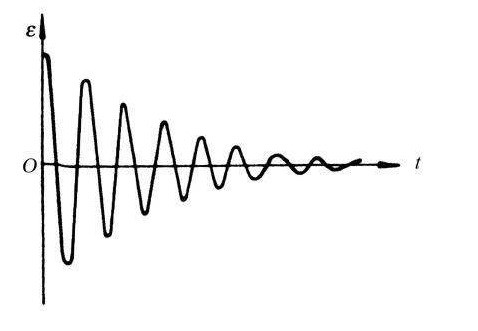
\includegraphics[width=\linewidth]{FID.jpg}
	\caption{Free Induction Decay}
	\label{fig:results}
\end{figure}
\par 通过FFT(Fast Fourier Transform)技术,我们就可以得到原子进动的角频率,进而计算出装置转动的角速度。
